\documentclass[12pt,a4paper]{jarticle}
\usepackage[top=35truemm, bottom=35truemm, left=30truemm, right=30truemm]{geometry}
\usepackage[dvipdfmx]{graphicx}
\setcounter{tocdepth}{\maxdimen} %subsubsectionまで目次を表示する
\bibliographystyle{junsrt} %参照のスタイル

\begin{document}
\begin{titlepage}
\title{\vspace{60mm} \LARGE 修士論文\vspace{10mm}\\J-PARC E07実験におけるbeam照射及び\\原子核乾板中の$\Xi$-粒子飛跡自動追跡}
\author{\Large 岐阜大学大学院 教育学研究科 \\ \vspace{5mm}
\Large 総合教科教育専攻 仲澤研究室 \\ \vspace{5mm}
\LARGE 後藤 良輔}
\date{最終更新 \today}
\maketitle
\thispagestyle{empty} %ページ番号を消す
\end{titlepage}

\thispagestyle{empty} %ページ番号を消す
\tableofcontents
\newpage
\section{序論}
\subsection{はじめに}
私たちを含め、身の回りの物質は原子からできている。その原子核は原子核と電子から構成されており、原子核は陽子と中性子で成り立つ。さらに、陽子や中性子はクォークで構成されている。\par
クォークは、up(u)、down(d)、strange(s)、charm(c)、top(t)、bottom(b)の6種類がある。(以降は()内の文字で省略する。)また、クォークには反対の電荷をもつ反クォークも存在する。この反クォークも6種類存在している。私たちはsクォークを持つ粒子の相互作用を研究の対象にしている。\par
一般に粒子の相互作用を調べるためには粒子同士の衝突散乱実験を行うが、私たちが実験で使用する$\Lambda$粒子寿命は$10^{-10}$秒と寿命が非常に短いため通常の方法で相互作用を知ることは不可能である。そのため、$\Lambda$粒子の相互作用を求めるには原子核の中に$\Lambda$粒子持つものを生成し、核の崩壊過程から相互作用を求めるという手法しかない。\par
私たちは原子核乾板という検出器を用いることで核の生成崩壊事象を記録し、崩壊事象から$\Lambda$粒子の相互作用を求めることを試みている。\par
\subsection{Double-$\Lambda$Hyper核}
通常の核に$\Lambda$粒子を2つ持たせたものがDouble-$\Lambda$Hyper核である。\par
$\Lambda$粒子はK$^+$K$^-$反応により生成する。\par
式をここに入れる。
\subsection{原子核乾板}
原子核乾板とは非常に高感度な写真フィルムの一種で、荷電粒子の通過した跡を記録する検出器である。私たちが実験で使用する$\Lambda$粒子の寿命は非常に短いため、Hyper核の生成・崩壊事象をすべて記録できる原子核乾板を使う必要がある。\par
原子核乾板の利点としては大きく分けて2点ある。\par
一点目は、現像処理を行うことで半永久的に顕微鏡による観測を可能にすることである。原子核乾板中を荷電粒子が通ることで、原子核乾板の主成分であるAgBrが電離され銀原子が生成される。現像処理により、銀が成長し1µm程度の粒となり(grain)、荷電粒子の飛跡がgrainの連なり(飛跡、track)として現れ、その状態を保持する。そのため、原子核乾板を破損しない限り一度記録したHyper核の生成・崩壊事象やHyper核以外の荷電粒子秘跡を何度でも同じ状態で観測することができる。\par
\begin{figure}[htbp]
 \begin{center}
  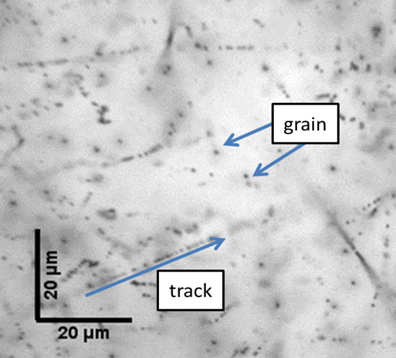
\includegraphics[width=70mm]{grainfog.png}
 \end{center}
 \caption{原子核乾板中に記録されるtrackとgrainの様子}
\end{figure}
二点目は、サブミクロン精度での空間分解能を持つことである。乾板に記録された飛跡の長さ、太さは通過した荷電粒子のエネルギーや電荷に依存する。そのため、私たちは$\Lambda$-$\Lambda$間に働く相互作用を記録されたHyper核事象の飛跡の長さと角度からエネルギーを計算することで算出することができる。\par
原子核乾板はBaseにEmulsionを塗布して作成している。Baseとはポリスチレンフィルムで作られた支持体である。Emulsionは通常の写真乳剤よりもハロゲン化銀の含有量が高く,最小電離損失に対して感度を持っているものである。E07実験で使用する原子核乾板1400枚(薄型:200、厚形:1200)はすべて岐阜大学で製造された。\par
乾板に飛跡が記録される際の流れの図\par
E07実験で使用する乾板は40µmのBaseに450µmの乳剤を塗布する厚型乾板と、180µmのBaseに100µmの乳剤を塗布する薄型乾板の二種類である。\par
乾板の規格の図\par
薄型乾板はSSDとemulsionとの接続に使用される。薄型乾板はbaseが厚く、乳剤が薄く塗布されているため現像の前後で乾板の変形が小さい。そのため、記録された飛跡の角度や位置を明確に求められる。\par
厚形乾板は照射された$\Xi$粒子を乾板中で静止させ、娘粒子の飛跡を記録するために用いられる。
\subsection{光学顕微鏡}
光学顕微鏡を用いて、現像後の原子核乾板に記録されているtrackを追跡・観察する。使用する顕微鏡は、モーターによって水平方向(x、y方向)に約1µmの精度で位置制御し、エンコーダーによって鉛直方向(z方向)に約0.1µmの精度で稼働できる。この顕微鏡により、原子核乾板表面の推測される位置で目的のtrackを探し、$\Xi$$^-$粒子候補を見つけ、trackを原子核乾板上面から下面まで追跡していく。\par
PCを接続することで、この光学顕微鏡を制御している。CCDカメラを顕微鏡に設置することで、顕微鏡で観察したものを画像として取得する。取得した画像をPCの画面上に表示することや、顕微鏡の稼働に活用している。$\Xi$$^-$粒子自動追跡には、50倍の対物レンズを使用している。使用する顕微鏡とPCを示す。
\subsection{KEK-PS E373実験}
\begin{itemize}
    \item この実験で●例のハイパー核事象が検出された。
    \item 検出されたイベントの例としては、Nagara、Kisoがある。
\end{itemize}
\subsection{J-PARC E07実験}
\begin{itemize}
    \item ハイブリッド方によりE373の10倍の統計、全面探査により100倍の統計を目指す実験である。
    \item 実験セットアップを示す。
    \item SSDに変更したことで、検出した候補の角度分解能、位置分解の精度が向上している。
    \item 10倍の統計になる、100倍の統計になる根拠を記入する。
\end{itemize}

\newpage
\section{J-PARC E07実験2ndRun}
\subsection{Refresh処理の実施}
\subsubsection{実施背景}
\begin{itemize}
 \item 放射能漏れで乾板を制作した直後にbeam照射ができなかった。
 \item 莫大なバックグラウンドの増加を防ぐため神岡鉱山内にて制作した原子核乾板を保管
 \item 神岡内で保管したことで岐阜大で保管するよりバックグラウンドの増加を押さえることができた。
 \item しかし、解析に支障が出る程度まで蓄積されたため、リフレッシュ処理を実施した。
 \item E07実験では1stRunで●枚、2ndRunで●枚のリフレッシュ処理を実施した。
\end{itemize}
J-PARCE07実験で移用する原子核乾板はすべて岐阜大学ダブルハイパー核実験棟にて制作した。制作は●~●の期間で完了している。\par
当初の予定では乾板製造後すぐにbeam照射を実施する予定であったが、J-PARCでの放射能漏れ事故により実験は延期なった。乾板の製造だけは上記の期間中に終了させたため、実験開始まで保管する必要が出てきた。岐阜大学内で保管をしても、宇宙船やコンプトンの影響を受け乾板にバックグラウンドが蓄積されていくため、莫大なバックグラウンドの増加を防ぐため、神岡鉱山内に製造した原子核乾板を保管することになった。
それにより岐阜大学内で保管した場合より非常に多くのバックグラウンドを削減することができた。しかし、製造からbeam照射まで2年の期間が経過したため、神岡鉱山内で保管していたとしても解析に支障を及ぼすレベルまでバックグラウンドが蓄積してしまった。そこで、原子核乾板に対して潜像退行処理(Refresh処理)を実施し、蓄積されたバックグラウンドの消去を試みた。
\subsubsection{原理}
\begin{itemize}
 \item 写真乾板には現像退行性がある。
 \item 高温・多湿の環境下に乾板を置くことでその性質を促進し記録されたバックグラウンドを消去することを現像退行性という。
 \item たくさんのD論も引用でいれるか。
\end{itemize}
\subsubsection{実施環境}
\begin{itemize}
 \item リフレッシュ処理を行うには温度●度、湿度●%の環境を●時間維持する必要がある。
 \item リフレッシュ処理を行うためその環境を維持する装置を作成した。
 \item 1stRunでは温度・湿度の調整を手動で行ってきたが、2ndRunでは温度・湿度の調整を自動で制御させた。[村本卒論]
 \item 湿度と厚みのグラフを載せて制御できていると書く。
\end{itemize}
\subsection{暗室の拡張}
\begin{itemize}
 \item 2ndRunではbeam照射後すぐにGridマークを照射するため、暗室を拡大する必要があった。
 \item 1stRunと2ndRunでの暗室とものの配置の違いを載せる。
\end{itemize}
2ndRunではbeam照射後の原子核乾板に対してJ-PARC内の暗室下でGridMark照射を実施した。そのため、2017年3月にGridMark照射装置を設置するため暗室の拡張を行った。\par
\subsection{GridMark照射}
\subsubsection{GridMarkネガ}
\begin{itemize}
 \item 1stRun乾板にはネガのつまり等もあり、Gridマークが照射されていない部分があったので、それを防ぐためにネガを新調した。
 \item 発注の注文図をつける。
\end{itemize}
1stRunではbeam照射後岐阜に乾板を郵送し、現像する数日前にGridMarkを照射した。これが原因か判明していないが、$\Xi$飛跡追跡の際に想定の精度で視野内に飛跡を持ってくることができなかった。また、2016年に実施されたE07実験testRunでbeam照射された原子核乾板に焼き付けられたGridマークがネガのつまり等で照射されていない等の問題が解消されないまま1stRunを行ったため、Gridマークが照射されていない箇所がある。これらを受けてネガの変更を行った。E07実験のと同様に発注し、ネガを貼り付けた。
\subsubsection{GridMark照射装置}
\begin{itemize}
 \item 1stRun乾板は人がストップウォッチを使い、10秒間露光すると言うことを●枚の乾板に対して実施した。
 \item この手法では1mod分照射するのに●時間が必要になるとともに、精神的疲労が大きいので変更した。
 \item 一瞬で●rpm?露光できるように作り替えた。
 \item 装置はこんな感じである。
\end{itemize}
E071stRunではタイマーを用いて10秒間原子核乾板に露光した。(田村卒論)参照論文と同様の手法で1mod分照射するのに約1時間半の時間が必要になるとともに時間をストップウォッチを使って計測していたため、多大な精神的疲労を負うことになっていた。\par
田村卒論を確認して、露光時間、最終的にどれくらい照射すれば良いのか、照射装置の構造の写真を引用して載せる。\par
E07実験2ndRunではbeam照射後すぐにGridマークを照射する。従来の手法から変更することで照射の時間短縮及び疲労の削減のために照射装置の改造を行った。
\subsection{E07実験beam照射}
\subsubsection{2ndRunbeam照射}
\begin{itemize}
 \item ●日をかけて原子核乾板●枚すべてにbeam照射を行った。
 \item beamライン等の図。Runendの図を見せて終了。
 \item 何日かけて実施したかを記す。照射Mod数/月日 の図
\end{itemize}
\subsubsection{岐阜大学の作業内容}
ここではemulsionカセットに乾板を詰める作業と乾板をカセットから出す。作業について書く。\par
遠藤修論を参考文献にする。
\begin{itemize}
 \item 乾板を冷蔵庫から出す。
 \item 袋から乾板を開けて乾板の重さ・厚さを測定し、乾板の番号を記録、乾板のMOD番号を書く。
\end{itemize}
\subsubsection{EmulsionCasetteでの真空度}
\begin{itemize}
 \item 遠藤修論にある基準をクリアすることを確認しながら実施。
 \item ある真空度グラフをのせ、適切に行えたということを示す。
 \item 残りのModに関しては付録にあると記す。
\end{itemize}
\subsubsection{照射した乾板の密度}
\begin{itemize}
 \item 乾板の密度は解析において非常に重要である。Nagaraの密度が違った場合のデータを見せる。
 \item カセットに入れる前と後で重さが大きく変化していないかを確認した。
 \item 測定した重さと厚さから乾板の密度を求めたところ、1stRunと2ndRunで密度の大きな違いは無かった。リフレッシュ処理の有無も乾板の密度測定には影響がなかったと言える。
\end{itemize}
原子核乾板中に記録されたHyper核eventを解析するためには記録されている原子核乾板の密度が重要になる。原子核乾板では記録された飛跡の飛程からエネルギーを算出する際に乾板の密度が必要になるからである。現在核種が一意に決定されている'NagaraEvent'の数値を使うとこのようなグラフになる。\par
このグラフから分かるように原子核乾板の密度を正確に求めることが必要である。\par
2ndRunでは1stRunと同様にemulsionCasetteに乾板を入れる前に乾板の厚さと重さの測定、beam照射後に乾板の重さを測定することでbeam照射により乾板の重さに大きな変動がないかを確認した。照射の前後で重さが1.0g以上異なっていた場合再度厚さ重さの測定をして記録した。乾板の重さは電子天秤で測定した。乾板の厚さはシックネスゲージを用いて乾板の4カ所を測定した。\par
この図は厚形乾板の1stRun乾板での密度の測定結果と2ndRun乾板での密度の測定結果である。比較すると、1stRunと2ndRunで使用した原子核乾板に大きな違いは無いように見える。また、1stRun乾板の密度はRefresh未処理の乾板、2ndRunはRefresh実施乾板での密度である。そのため、Refresh処理の有無で原子核乾板の密度が変化しないことが分かる。\par
薄型乾板でも同様に密度の比較をした。1stRunの薄型乾板は厚形乾板より密度が大きく算出されていたが、2ndRunで使用した薄型乾板でも同様の傾向になった。
\subsection{現像}
\begin{itemize}
 \item 原子核乾板すべて現像している。
 \item 現像の行程
 \item 1stRunは●年に●枚終了、2ndRunは●年に●枚終了予定
\end{itemize}



\newpage
\section{荷電粒子飛跡追跡の自動化}
\subsection{目的}
E373実験では人が非常に多くの$\Xi$$^-$候補を顕微鏡を使い静止点まで追跡した。この追跡には約数年が必要となった。先に記述したが、今年度実施されたJ-PARC E07実験はではE373実験の約10倍の統計量を検出することを目標にしている。E07実験にて採用されているハイブリッド方では、E373実験より精度の高い検出機であるSSDを使い追跡するべき飛跡候補を絞ることで追跡するべき飛跡を増やさないようにしている。しかしその条件であっても追跡すべき飛跡はE373実験の場合を超えるため、人が操作せずに機械が自動で静止点まで追跡するプログラムの作成が必要になった。\par
SSDとE373実験の際に使用された検出機の精度をまとめた表を示す。
\subsection{$\Xi$$^-$候補&beam認識に用いる画像処理}
\subsubsection{コントラスト処理}
\begin{itemize}
    \item 乾板の写真は撮影した地点によりコントラストが異なるので、撮影の位置によらず画像を同等に扱いたいのでコントラスト処理をかける。
    \item 位置による乾板中の飛跡の見え方の違いを示す。
    \item コントラスト処理で使用する数式を示す&それを説明した図を入れる。
    \item 処理前と処理後の画像を入れる。
\end{itemize}
\subsubsection{ガウシアンフィルタ処理}
\begin{itemize}
    \item 撮影された画像にはノイズが記録されているので、そのノイズを消すためにガウシアンフィルタ処理により画像をぼかす。
    \item ガウシアンフィルタ処理の数式を入れる。
    \item 処理前と処理後の画像を入れる。
\end{itemize}
\subsubsection{画像の白黒反転}
\begin{itemize}
    \item ガウシアンフィルタ処理とコントラスト処理をかけた画像の輝度値の差分を取ることで、白黒反転の画像を作成する。
    \item 今後の画像処理のために白黒反転処理を行う。
    \item 処理前と処理後の画像&なぜ白黒反転になるのかの図を入れる。
\end{itemize}
\subsubsection{二値化}
\begin{itemize}
    \item 白黒反転画像に対して、ある一定以上の輝度値をもつピクセルのみ残すという処理を行う。
    \item これによりある程度濃く記録された飛跡情報のみがのこるのでこのようにしている。飛跡のエネルギーが高いものは濃く記録されると言うことの図を入れた方が良いかも。
    \item 処理前と処理後の画像
\end{itemize}
\subsection{座標変換}
\subsection{自動追跡の要素技術}
\subsubsection{P-barパターンマッチ}
原子核乾板にはSSDとemulsionの照射時の位置差を取得するためにアンチプロトンbeamが照射されている。照射されているのは乾板の四つ角1cm1cmの領域である。照射されているp-barの濃度は1平方センチあたり10の4乗である。k-beamは乾板に対して10の6乗照射されており、SSDとemulsionのパターンマッチをするには密に照射されすぎているのでp-barが必要になる。\par
角から1cmずつ内陸側に移動し、そこで5mm×5mmの領域をスキャンする。上側乳剤層と下側乳剤層をスキャンし、baseを挟んで接続された垂直なbeamを使いパターンマッチを行う。\par
\subsubsection{$\Xi$$^-$候補飛跡の選択}
下流の乾板に接続して追跡するために、SSDで検出した$\Xi$$^-$候補とpl01に記録された荷電粒子飛跡の対応をつける。
\subsubsection{K$^-$beamパターンマッチ}
beam照射時の上流乾板と下流乾板の位置ずれを取得するために乾板に照射されているK$^-$beamを用いてパターンマッチを行う。
\subsubsection{表面認識}
\subsubsection{荷電粒子飛跡追跡}

\newpage
\section{E07乾板における開発プログラムの追跡実績}

\newpage
\section{まとめ}
\end{document}